% @Author: luis
% @Date:   2016-02-20 12:42:09
% @Last Modified by:   luis
% @Last Modified time: 2016-03-25 16:59:24

% @Author: Luis Perez
% @Date:   2016-02-02 21:09:55
% @Last Modified by:   luis
% @Last Modified time: 2016-02-19 17:47:15

\documentclass[12pt]{article}
\usepackage{latexsym}
\usepackage{fancyhdr}
\usepackage{amssymb,amsmath,amsthm}
\usepackage[pdftex]{graphicx}
\usepackage{pdfpages}
\usepackage{hyperref}
\usepackage[margin=1in]{geometry}


% Create answer counter to keep track of seperate responses
\newcounter{AnswerCounter}
\newcounter{SubAnswerCounter}
\newcounter{SubSubAnswerCounter}
\setcounter{AnswerCounter}{1}
\setcounter{SubAnswerCounter}{1}
\setcounter{SubSubAnswerCounter}{1}

% Create answer environment which uses counter
\newenvironment{answer}[0]{
  \setcounter{SubAnswerCounter}{1}
  \bigskip
  \textbf{Solution \arabic{AnswerCounter}}
  \\
  \begin{small}
}{
  \end{small}
  \stepcounter{AnswerCounter}
}

\newenvironment{subanswer}[0]{
  \setcounter{SubSubAnswerCounter}{1}
  (\alph{SubAnswerCounter})
}{
 \bigskip
  \stepcounter{SubAnswerCounter}
}

\newenvironment{subsubanswer}[0]{
  \hspace{0.25in}[\roman{SubSubAnswerCounter}]
}{
 \bigskip
  \stepcounter{SubSubAnswerCounter}
}

% Allows easy use of vectors
\newcommand{\vect}[1]{\boldsymbol{#1}}
\newcommand{\deln}[3]{\frac{\partial^{#3} #1}{\partial #2^{#3}}}
\newcommand{\del}[2]{\frac{\partial#1}{\partial #2}}
\newcommand{\bra}[1]{\langle {#1} |}
\newcommand{\ket}[1]{| {#1} \rangle}
\newcommand{\dt}[2]{\langle {#1} | {#2} \rangle}
\newcommand{\braket}[3]{\langle {#1} | {#2} | {#3} \rangle}
\newcommand{\op}[1]{{#1}_{op}}
\newcommand{\opb}[1]{{\bf {#1}}_{op}}


% Custom Header information on each page
\pagestyle{fancy}
\lhead{HUID: 70871564}
\rhead{Luis Perez - \thepage}
\renewcommand{\headrulewidth}{0.1pt}
\renewcommand{\footrulewidth}{0.1pt}

\newcommand{\horrule}[1]{\rule{\linewidth}{#1}}   % Horizontal rule
\title{
    % \vspace{-1in}
    \usefont{OT1}{bch}{b}{n}
    \normalfont \normalsize \textsc{Harvard University} \\ [25pt]
    \horrule{0.5pt} \\[0.4cm]
    \huge Physics 143a: Quantum Mechanics I \\ [20pt]
    \normalfont \normalsize Problem Set 6
    \horrule{2pt} \\[0.5cm]
}
\author{
    \normalfont                 \normalsize
        Luis Antonio Perez\\[-3pt]    \normalsize
}
\date{\today}

\begin{document}
\maketitle
\pagebreak

\begin{answer}
We now consider our old friend, the general two state system with Hamiltonian $H_0$ and eigenstates $\ket{1}$ and $\ket{2}$ with eigenvalues $E_1, E_2$ respectively. Note that the most general wave function is the super position $\ket{\psi} = c_1 \ket{1} + c_2 \ket{2}$.

\begin{subanswer}
We can write the Hamiltonian $H_0$ in Dirac notations as follows:
$$
H_0 = E_1 \ket{1}\bra{1} + E_2\ket{2}\bra{2}
$$
Note that this is just the combination of the identity operator for the $n$-th eigenstate ($\ket{n}\bra{n}$) scaled by the respective eigenvalue. We can verify the Hamiltonian behaves as expected:
$$
H_0\ket{1} = E_1 \ket{1}\dt{1}{1} + E_2\ket{2}\dt{2}{1} = E_1\ket{1}
$$
$$
H_0\ket{2} = E_1 \ket{1}\dt{1}{2} + E_2\ket{2}\dt{2}{2} = E_2\ket{2}
$$
We can also represent $H$ as a matrix with matrix elements given by:
\begin{align*}
\braket{1}{H_0}{1} = E_1 \\
\braket{2}{H_0}{2} = E_2 \\
\braket{1}{H_0}{2} = 0 \\
\braket{2}{H_0}{1} = 0
\end{align*}
so in the basis given by the eigenstates ($\mathcal{B} = \{\ket{1}, \ket{2}\}$, $H$ can be viewed as the matrix:
$$
H_0 = \begin{pmatrix} E_1 & 0 \\ 0 & E_2 \end{pmatrix}
$$
Note that the correct definition, however, involves defining the matrix elements for some arbitrary basis $\mathcal{B}'$, which can be done by letting $B$ be the matrix transformation from $\mathcal{B} \to \mathcal{B}'$ (which we can explicitly construct by taking each column in $B$ to be one of our basis elements), and then the Hamiltonian in the $\mathcal{B}'$ basis is given by:
$$
H_0' = B H_0 B^\dag
$$
However, the above is just a generalized statement of the matrix-element property:
$$
H_0 = \begin{pmatrix} \braket{1}{H_0}{1} & \braket{1}{H_0}{2} \\ \braket{2}{H_0}{1} &\braket{2}{H_0}{2} \end{pmatrix}
$$
\end{subanswer}

\begin{subanswer}
We can define the most general time-dependent state of this system using Dirac by adding the standard time-dependence to each of the eigenstates (we assume $a_i$ is complex so we don't have to explicitly deal with phase factors):
$$
\ket{\Psi(t)} = a_1e^{-i E_1 t / \hbar}\ket{1} + a_2 e^{-i E_2 t/  \hbar}\ket{2}
$$
which can be represented as well in the convention of matrix quantum mechanics for some arbitrary basis $\mathcal{B} = \{\ket{-},\ket{+}\}$ as:
$$
\ket{\Psi(t)} = \begin{pmatrix}
a_1e^{-i E_1 t / \hbar}\dt{+}{1} + a_2 e^{-i E_2 t/  \hbar}\dt{+}{2}\\
a_1e^{-i E_1 t / \hbar}\dt{-}{1} + a_2 e^{-i E_2 t/  \hbar}\dt{-}{2}
\end{pmatrix}
$$
which, assuming a representation of the matrix in the energy eigenstates basis (ie, $\ket{-} = \ket{2}$ and $\ket{+} = \ket{1}$, we can simplify to:
$$
\ket{\Psi(t)} =
\begin{pmatrix} a_1e^{-i E_1 t / \hbar} \\
a_2e^{-i E_2 t / \hbar}
\end{pmatrix}
$$
\end{subanswer}

\begin{subanswer}
We now calculate how how the probability that the system is between $x$ and $x + dx$ varies with time by directly computing $|\Psi(t)|^2 = \Psi(t)^*\Psi(t) =  \dt{\Psi(t)}{x}\dt{x}{\Psi(t)}$. For practice, we do this in Diract notation using the position representation.
\begin{align*}
\dt{\Psi(t)}{x}\dt{x}{\Psi(t)} &= [a_1^*e^{i E_1 t / \hbar}\dt{1}{x} + a_2^* e^{i E_2 t/  \hbar}\dt{2}{x}][a_1e^{-i E_1 t / \hbar}\dt{1}{x} + a_2 e^{-i E_2 t/  \hbar}\dt{2}{x}] \\
&= |a_1|^2 \dt{1}{x}\dt{x}{1} + |a_2|^2 \dt{2}{x}\dt{x}{2} + a_1^*a_2 e^{i(E_1 - E_2) t / \hbar}\dt{1}{x}\dt{x}{2} + a_1a_2^* e^{i(E_2 - E_1) t / \hbar} \dt{2}{x}\dt{x}{1}
\end{align*}
which cannot be further simplified unless we integrate over the entire space, in which case using the identity that $1 = \int dx \ket{x}\bra{x}$ and orthonormality of $\ket{1},\ket{2}$ we can achieve simplifications. Note that we could have also used the momentum representation or the energy representation (which we calculate below), but for consistency we took advantage of the position representation where $\ket{x}$ is an eigenket of the position operator $x_{op}$.
\end{subanswer}

\begin{subanswer}
The Hamiltonian for the modified system is given by:
$$
H = H_0 + V
$$
where we note that $V$ can be written in Diract notation as:
$$
V = v\ket{1}\bra{2} + v\ket{2}\bra{1} =  v(\ket{1}\bra{2} + \ket{2}\bra{1})
$$
and therefore we have:
$$
H = E_1 \ket{1}\bra{1} + E_2\ket{2}\bra{2} + v(\ket{1}\bra{2} + \ket{2}\bra{1})
$$
We can represent the above in matrix notation by noting that the matrix elements of the new Hamiltonian are now, in the energy eigenket basis:
\begin{align*}
H &= \begin{pmatrix} \braket{1}{H}{1} & \braket{1}{H}{2} \\ \braket{2}{H}{1} &\braket{2}{H}{2} \end{pmatrix} \\
&= \begin{pmatrix} \braket{1}{[E_1 \ket{1}\bra{1} + E_2\ket{2}\bra{2} + v(\ket{1}\bra{2} + \ket{2}\bra{1})]}{1} & \braket{1}{[E_1 \ket{1}\bra{1} + E_2\ket{2}\bra{2} + v(\ket{1}\bra{2} + \ket{2}\bra{1})]}{2} \\ \braket{2}{[E_1 \ket{1}\bra{1} + E_2\ket{2}\bra{2} + v(\ket{1}\bra{2} + \ket{2}\bra{1})]}{1} &\braket{2}{[E_1 \ket{1}\bra{1} + E_2\ket{2}\bra{2} + v(\ket{1}\bra{2} + \ket{2}\bra{1})]}{2} \end{pmatrix} \\
&= \begin{pmatrix}
E_1 & v \\
v & E_2
\end{pmatrix}
\end{align*}
\end{subanswer}

\begin{subanswer}
The TISE for the modified system is as follows:
\begin{align*}
H \ket{\psi} &= a_1 H \ket{1} + a_2 H \ket{2} \\
&=a_1[E_1 \ket{1}\dt{1}{1} + E_2\ket{2}\dt{2}{1} + v(\ket{1}\dt{2}{1} + \ket{2}\dt{1}{1})] + a_2[E_1 \ket{1}\dt{1}{2} + E_2\ket{2}\dt{2}{2} + v(\ket{1}\dt{2}{2} + \ket{2}\dt{1}{2})] \\
&= a_1 E_1 \ket{1} + a_1v\ket{2} + a_2E_2\ket{2} + a_2v\ket{1}\\
&= (a_1E_1 + a_2v)\ket{1} + (a_2E_2 + a_1v)\ket{2} \\
&= \mathcal{E}\ket{\psi} \\
&= \mathcal{E}(a_1 \ket{1} + a_2 \ket{2}) \\
&= a_1\mathcal{E}\ket{1} + a_2\mathcal{E}\ket{2}
\end{align*}
where we made use of the fact that the eigenstates are orthonormal. This lead to the final equations:
$$
(a_1E_1 + a_2v)\ket{1} + (a_2E_2 + a_1v)\ket{2} = a_1\mathcal{E}\ket{1} + a_2\mathcal{E}\ket{2}
$$
We can also perform the same operations using the matrix representation of quantum mechanics to arrive at the matrix equation (we assume the basis consists of $\{\ket{1}, \ket{2} \}$ to avoid the cumbersome notation of transforming from an arbitrary basis):
\begin{align*}
H\ket{\psi} &= \begin{pmatrix} E_1 & v \\ v & E_2 \end{pmatrix}\begin{pmatrix}  a_1\\ a_2 \end{pmatrix} \\
&= \mathcal{E}\begin{pmatrix} a_1 \\ a_2 \end{pmatrix}
\end{align*}
\end{subanswer}

\begin{subanswer}
Note that in order for the Dirac notation to hold, we must have that:
$$
a_1E_1 + a_2v = a_1 \mathcal{E}
$$
$$
a_2E_2 + a_1v = a_2 \mathcal{E}
$$
which can be written as the matrix equation:
\begin{align*}
\begin{pmatrix} E_1 & v \\ v & E_2 \end{pmatrix}\begin{pmatrix}  a_1\\ a_2 \end{pmatrix}
&= \mathcal{E}\begin{pmatrix} a_1 \\ a_2 \end{pmatrix}
\end{align*}
which coincides with the matrix representation of the SE derived previously (this is good news!). We can then transform this into a homogeneous matrix equations by subtracting off the vector $\mathcal{E}\begin{pmatrix}a_1 \\ a_2 \end{pmatrix}$ and then factoring out the vector by inserting the identity matrix to yield:
$$
\begin{pmatrix} E_1 - \mathcal{E} & v \\ v & E_2 - \mathcal{E}\end{pmatrix} \begin{pmatrix} a_1 \\ a_2\end{pmatrix}= 0
$$
\end{subanswer}

\begin{subanswer}
Using the results from above, the system has non-trivial solutions $\iff$ the final matrix above has a non-empty null-space (aka, the kernel is non-empty). This will be the case $\iff$ the determinant is equal to $0$. This yields the equations:
\begin{align*}
&\det \begin{pmatrix} E_1 - \mathcal{E} & v \\ v & E_2 - \mathcal{E}\end{pmatrix} = 0 \\
\implies& (E_1 - \mathcal{E})(E_2 - \mathcal{E}) - v^2 = 0
\end{align*}
which must hold for non-trivial solutions to exists.
\end{subanswer}

\begin{subanswer}
We can now solve the above equation for the unknown $\mathcal{E}$:
\begin{align*}
&(E_1 - \mathcal{E})(E_2 - \mathcal{E}) - v^2 = 0 \\
\implies& \mathcal{E}^2 - (E_1 + E_2)\mathcal{E} + E_1E_2 - v^2 = 0 \\
\implies & \left(\mathcal{E} - \frac{E_1 + E_2}{2}\right)^2 = \frac{(E_1 + E_2)^2}{4} - E_1E_2 + v^2 \\
\implies & \mathcal{E}_{\pm} - \frac{E_1 + E_2}{2} = \pm \frac{1}{2}\sqrt{(E_1 + E_2)^2 - 4E_1E_2 + 4v^2} \\
\implies & \mathcal{E}_{\pm}  = \frac{1}{2}\left[E_1 + E_2\pm \sqrt{(E_1 - E_2)^2 + 4v^2}\right]
\end{align*}
\end{subanswer}

\begin{subanswer}
We now calculate energy eigenkets when $v = 0$. We have:
$$
\mathcal{E}_{\pm} = \frac{1}{2}[E_1 + E_2 \pm (E_1 - E_2)]
$$
which gives two energy eigentkets, $\ket{\mathcal{E}_-}$ and $\ket{\mathcal{E}_+}$ with eigenvalues $E_2$ and $E_1$ respectively. That is to say, they satisfy the following:
$$
H\ket{\mathcal{E}_-} = E_2\ket{\mathcal{E}_-}
$$
$$
H\ket{\mathcal{E}_+} = E_1 \ket{\mathcal{E}_+}
$$
therefore the energy eignekets are simply $\ket{\mathcal{E}_-} = \ket{2}$ and $\ket{\mathcal{E}_+} = \ket{1}$.
\end{subanswer}

\begin{subanswer}
We now calculate energy eigenkets when $v \to \infty$. Note that in this case, $4v^2 >> (E_1 - E_2)^2$ and $v >> E_1 + E_2$, so we can ignore that term under the square root. This results in:
$$
\mathcal{E}_{\infty_\pm} \approx \frac{1}{2}[E_1 + E_2 \pm 2v] \approx \pm v
$$
for very large $v$ since we can ignore the constants $E_1 + E_2$ and $(E_1 - E_2)^2$. This given the energy eigenkets with the following properties:
$$
H\ket{\mathcal{E}_{\infty_+}} = v\ket{\mathcal{E}_{\infty_+}}
$$
$$
H\ket{\mathcal{E}_{\infty_-}} = -v\ket{\mathcal{E}_{\infty_-}}
$$
though note that as $v \to \infty$, the eigenvalues diverge to $+\infty$ and $-\infty$ respectively.
\end{subanswer}

\begin{subanswer}
We now calculate energy eigenkets when $v \to -\infty$. Note that in this case, $4v^2 >> (E_1 - E_2)^2$ and $-v >> E_1 + V_2$, so we can ignore that term under the square root. This results in:
$$
\mathcal{E}_{\infty_\pm} \approx \frac{1}{2}[E_1 + E_2 \pm 2v] \approx \pm v
$$
for very large $v$ since we can ignore the constants $E_1 + E_2$ and $(E_1 - E_2)^2$. This given the energy eigenkets with the following properties:
$$
H\ket{\mathcal{E}_{-\infty_+}} = v\ket{\mathcal{E}_{\infty_+}}
$$
$$
H\ket{\mathcal{E}_{-\infty_-}} = -v\ket{\mathcal{E}_{\infty_-}}
$$
though note that as $v \to -\infty$, the eigenvalues diverge to $-\infty$ and $+\infty$ respectively.
\end{subanswer}

\begin{subanswer}
Figure \ref{fig:energies} shows the required plot. Note that the graphs have the property that as $v \to \infty$, they asymptotically approach the line $\mathcal{E}_{\pm} = \pm v$ and as $v \to -\infty$ they asymptotically approach the line $\mathcal{E}_{\pm} = \mp v$

\begin{figure}[h!]
\centering
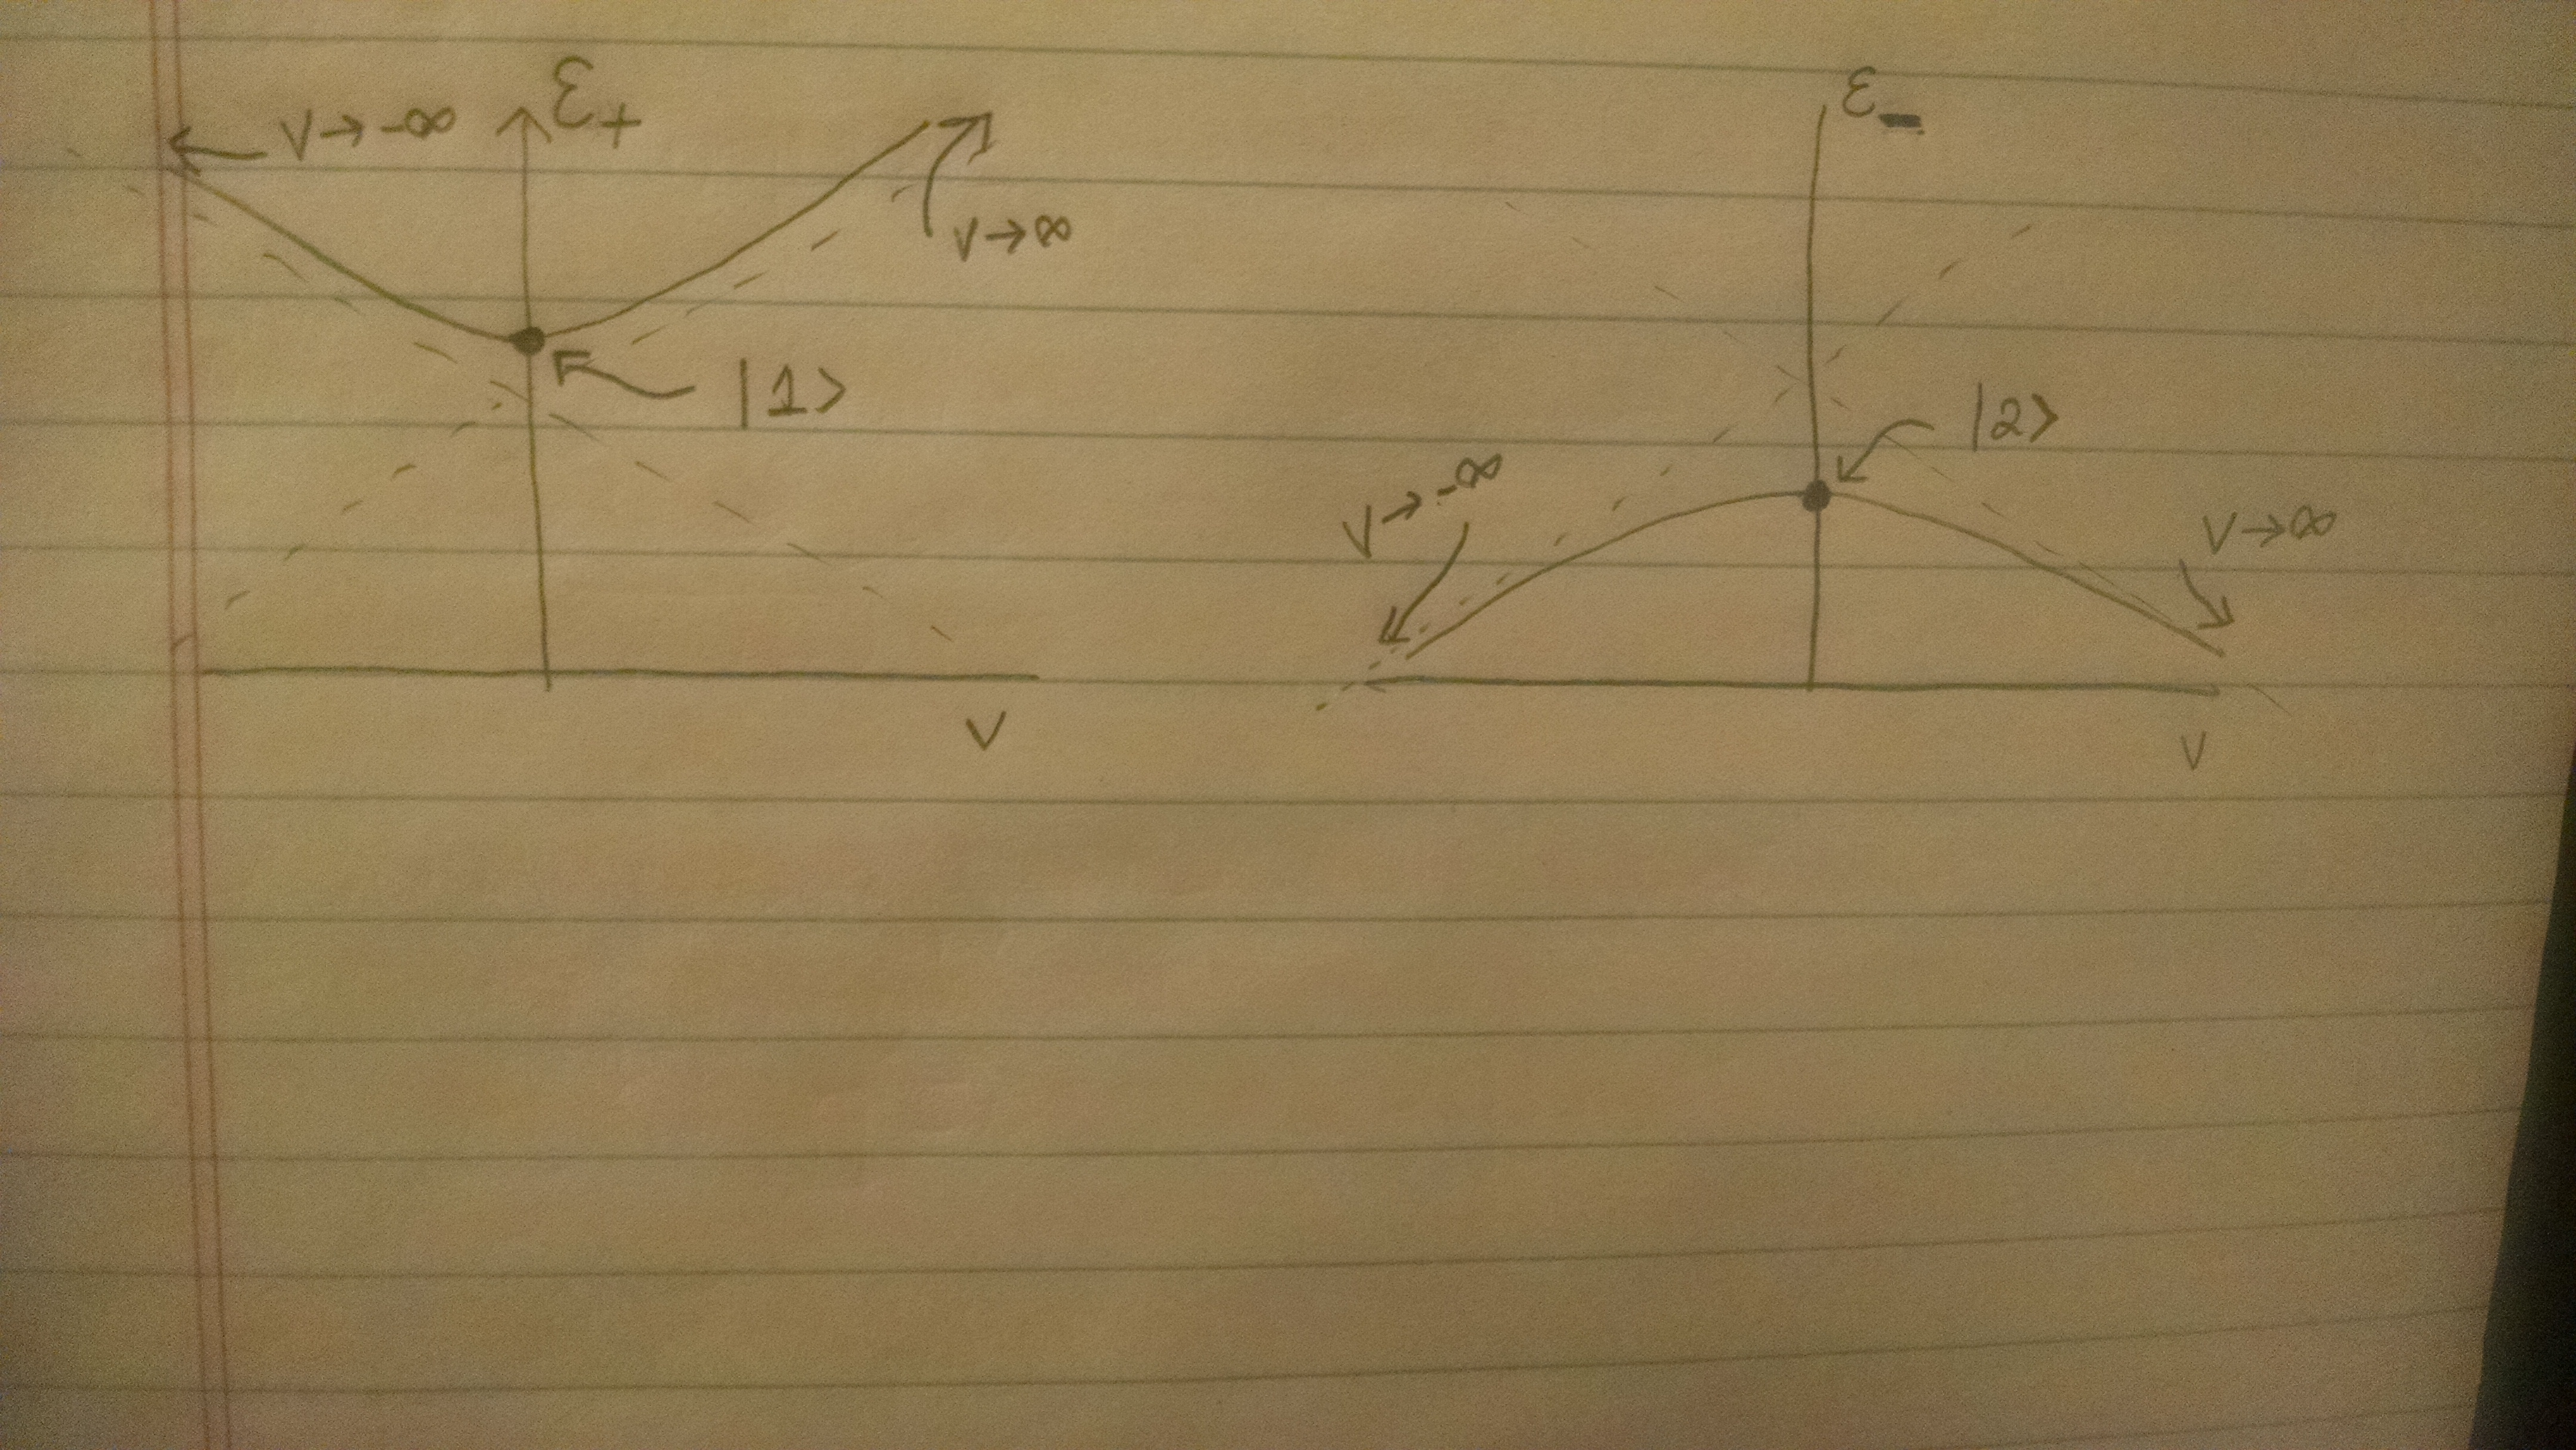
\includegraphics[scale=.07]{plot_energies.jpg}
\label{fig:energies}
\caption{Plot of $\mathcal{E}_+$ and $\mathcal{E}_-$ assuming that $E_1 > E_2$ with labeled eigenkets.}
\end{figure}
\end{subanswer}
\end{answer}

\begin{answer}
We consider potential energies $V(x)$ which can be expanded as a power series $\sum_{j} b_k x^{j}$ so that we can then define $V_{op} = V(x_{op})$. With this in mind, we now consider the SE:
$$
i\hbar \del{}{t}\ket{\psi(t)} = H_{op}\ket{\psi(t)}
$$
under different representations (momentum and configuration space). Note that $H_{op} = \frac{p_{op}^2}{2m} + V_{op}$.

\begin{subanswer}
We consider the configuration space representation. The equation under this representation becomes:
$$
\braket{x}{i\hbar \del{}{t}}{\psi(t)} = \braket{x}{\frac{p_{op}^2}{2m} + V_{op}}{\psi(t)}
$$
From this point forward, to simplify notation, we drop the $op$ subscript as well as the $t$ parameter. We can assume their existence from context.
We begin by simplifying the left hand since. First, we take a look at $\braket{\psi(t)}{i\hbar \del{}{t}}{\psi(t)}$ and note two possible relations.
\begin{align*}
\braket{\psi}{i\hbar \del{}{t}}{\psi} &= \int dx \dt{\psi}{x}\underbrace{\braket{x}{i \hbar \del{}{t}}{\psi}}_{\text{we're looking for this}} \\
\braket{\psi}{i\hbar \del{}{t}}{\psi} &= \int \int dx dx' \dt{\psi}{x}\braket{x}{i \hbar \del{}{t}}{x'}\dt{x'}{\psi}
\end{align*}
If we simplify the second equation above, we have the following:
\begin{align*}
\int \int dx dx' \dt{\psi}{x}\braket{x}{i \hbar \del{}{t}}{x'}\dt{x'}{\psi} &= \int \int dx dx' \dt{\psi}{x}\dt{x}{x'}(i \hbar \del{}{t}\dt{x'}{\psi}) \\
&= \int dx \dt{\psi}{x} \int dx' \dt{x}{x'}(i \hbar \del{}{t}\dt{x'}{\psi}) \\
&= \int dx \dt{\psi}{x} \int dx' \delta(x - x')(i \hbar \del{}{t}\dt{x'}{\psi}) \\
&=\int dx \dt{\psi}{x} (i \hbar \del{}{t}\dt{x}{\psi})
\end{align*}
By comparing this simplified second equation to the first, we can conclude that:
$$
\braket{x}{i \hbar \del{}{t}}{\psi} = i \hbar \del{}{t}\dt{x}{\psi}
$$
Next, we focus on calculating the RHS of the equation. Note that we can split the calculation into two parts - the potential energy and the kinetic energy. Tackling the potential energy, we first take note of the following fact:
$x_{op}^0 = I$ where $I$ is the identity operator. Therefore $\braket{\alpha}{x_{op}^0}{\beta} = \dt{\alpha}{\beta}$. This fact is used at the last step of the simplification.
\begin{align*}
\braket{x}{V_{op}}{\psi} &= \braket{x}{\sum_j b_j x_{op}^j}{\psi} \\
&= \sum_j b_j \braket{x}{x^j_{op}}{\psi}
\end{align*}
Calculating the inner summand:
\begin{align*}
\braket{x}{x^j_{op}}{\psi} &= \int dx' \braket{x}{x_{op}}{x'} \braket{x'}{x^{j-1}_{op}}{\psi} \\
&= \int dx' x \delta(x - x') \braket{x'}{x^{j-1}_{op}}{\psi} \\
&= x  \braket{x}{x^{j-1}_{op}}{\psi} \\
&= \cdots \\
&= x^j \braket{x}{x_{op}^0}{\psi}\\
& = x^j \dt{x}{\psi}
\end{align*}
so we conclude that:
$$
\braket{x}{V_{op}}{\psi} = \left(\sum_j b_j x^j \right)\dt{x}{\psi}
$$
Now we calculate the kinetic operator using a similar technique:
\begin{align*}
\braket{x}{p_{op}^2}{\psi} &= \int dx' \braket{x}{p_{op}}{x'}\braket{x'}{p_{op}}{\psi} \\
&= -i\hbar \int dx' \delta'(x - x')\braket{x'}{p_{op}}{\psi} \\
&= -i\hbar \del{}{x}\braket{x}{p_{op}}{\psi} \\
&= -i\hbar \del{}{x}\int dx' \braket{x}{p_{op}}{x'}\dt{x'}{\psi} \\
&= -\hbar^2 \deln{}{x}{2}\dt{x}{\psi}
\end{align*}
which then leads us to the conclusion that:
$$
\braket{x}{\frac{p_{op}^2}{2m}}{\psi} = \frac{\braket{x}{p_{op}^2}{\psi}}{2m} = -\frac{\hbar^2}{2m}\deln{}{x}{2}\dt{x}{\psi}
$$
and putting it all together we have the SE equation in the configuration position representations as:
$$
i\hbar \del{}{t}\dt{x}{\psi} = \left[-\frac{\hbar}{2m}\deln{}{x}{2} +  \sum_j b_j x^j \right]\dt{x}{\psi}
$$
\end{subanswer}

\begin{subanswer}
We consider the momentum representation. The equation under this representation becomes:
$$
\braket{p}{i\hbar \del{}{t}}{\psi(t)} = \braket{p}{\frac{p_{op}^2}{2m} + V_{op}}{\psi(t)}
$$
From this point forward, to simplify notation, we drop the $op$ subscript as well as the $t$ parameter. We can assume their existence from context.
We begin by simplifying the left hand since. First, we take a look at $\braket{\psi(t)}{i\hbar \del{}{t}}{\psi(t)}$ and note two possible relations.
\begin{align*}
\braket{\psi}{i\hbar \del{}{t}}{\psi} &= \int dp \dt{\psi}{p}\underbrace{\braket{p}{i \hbar \del{}{t}}{\psi}}_{\text{we're looking for this}} \\
\braket{\psi}{i\hbar \del{}{t}}{\psi} &= \int \int dp dp' \dt{\psi}{p}\braket{p}{i \hbar \del{}{t}}{p'}\dt{p'}{\psi}
\end{align*}
If we simplify the second equation above, we have the following:
\begin{align*}
\int \int dp dp' \dt{\psi}{p}\braket{p}{i \hbar \del{}{t}}{p'}\dt{p'}{\psi} &= \int \int dp dp' \dt{\psi}{p}\dt{p}{p'}(i \hbar \del{}{t}\dt{p'}{\psi}) \\
&= \int dp \dt{\psi}{p} \int dp' \dt{p}{p'}(i \hbar \del{}{t}\dt{p'}{\psi}) \\
&= \int dp \dt{\psi}{p} \int dp' \delta(p - p')(i \hbar \del{}{t}\dt{p'}{\psi}) \\
&=\int dp \dt{\psi}{p} (i \hbar \del{}{t}\dt{p}{\psi})
\end{align*}
By comparing this simplified second equation to the first, we can conclude that:
$$
\braket{p}{i \hbar \del{}{t}}{\psi} = i \hbar \del{}{t}\dt{p}{\psi}
$$
Next, we focus on calculating the RHS of the equation. Note that we can split the calculation into two parts - the potential energy and the kinetic energy. Tackling the potential energy, we first take note of the following fact:
$x_{op}^0 = I$ where $I$ is the identity operator. Therefore $\braket{\alpha}{x_{op}^0}{\beta} = \dt{\alpha}{\beta}$. This fact is used at the last step of the simplification.
\begin{align*}
\braket{p}{V_{op}}{\psi} &= \braket{p}{\sum_j b_j x_{op}^j}{\psi} \\
&= \sum_j b_j \braket{p}{x^j_{op}}{\psi}
\end{align*}
Calculating the inner summand:
\begin{align*}
\braket{p}{x^j_{op}}{\psi} &= \int dp' \braket{p}{x_{op}}{p'} \braket{p'}{x^{j-1}_{op}}{\psi} \\
&= \int dp' i\hbar \delta'(p - p') \braket{p'}{x^{j-1}_{op}}{\psi} \\
&= i\hbar  \del{}{p}\braket{p}{p^{j-1}_{op}}{\psi} \\
&= \cdots \\
&= (i\hbar)^j \deln{}{p}{j}\braket{p}{x_{op}^0}{\psi}\\
& = (i\hbar)^j \deln{}{p}{j}\dt{p}{\psi}
\end{align*}
so we conclude that:
\begin{align*}
\braket{p}{V_{op}}{\psi} &= \left(\sum_j b_j i^j\hbar^j \deln{}{p}{j}\right)\dt{p}{\psi} \\
&= \left(\sum_{j=0}^{\infty} \hbar^{4j}[b_{4j} - b_{4j + 2}\hbar^{2}\deln{}{p}{2} + i\hbar\del{}{p}(b_{4j + 1} - b_{4j+3}\hbar^2\deln{}{p}{2})]\deln{}{p}{4j} \right) \dt{p}{\psi}
\end{align*}
Now we calculate the kinetic operator using a similar technique:
\begin{align*}
\braket{p}{p_{op}^2}{\psi} &= \int dp' \braket{p}{p_{op}}{p'}\braket{p'}{p_{op}}{\psi} \\
&= p \int dp' \delta(p - p')\braket{p'}{p_{op}}{\psi} \\
&= p \braket{p}{p_{op}}{\psi} \\
&= p \int dp' \braket{p}{p_{op}}{p'}\dt{p'}{\psi} \\
&= p^2 \dt{p}{\psi}
\end{align*}
which then leads us to the conclusion that:
$$
\braket{p}{\frac{p_{op}^2}{2m}}{\psi} = \frac{\braket{p}{p_{op}^2}{\psi}}{2m} = \frac{p^2}{2m}\dt{p}{\psi}
$$
and putting it all together we have the SE equation in the configuration position representations as:
$$
i\hbar \del{}{t}\dt{p}{\psi} = \left[\frac{p^2}{2m} +  \sum_j b_j i^j\hbar^j \deln{}{p}{j}\right]\dt{p}{\psi}
$$
(note that we can also substitute the slightly simplified sum expression where we try to tease apart the behavior of $i^j$).
\end{subanswer}
\end{answer}

\begin{answer}
Note that an operator is Hermitian with $A^\dag = A$ only if this statement is true for all states in the Hilbert space (ie, for arbitrary $\psi,\phi$, we have that $\braket{\psi}{A^\dag}{\phi} = \braket{\psi}{A}{\phi}$).

\begin{subanswer}
We show that $x_{op}$ is Hermitian in both the position and momentum representations. First, we tackle the position representations. First, take arbitrary $\ket{\psi}$ and $\ket{\phi}$ and note:
\begin{align*}
\braket{\psi}{x_{op}^\dag}{\phi} &= \int \int dx dx' \dt{\psi}{x}\braket{x}{x_{op}^\dag}{x'}\dt{x}{\phi} \tag{using $1 = \int dy \ket{y}\bra{y}$ twice} \\
&= \int \int dx dx' \dt{\psi}{x}\braket{x'}{x_{op}}{x}^*\dt{x}{\phi} \tag{complex conjugate} \\
&= \int \int dx dx' \dt{\psi}{x}(x \delta(x' - x))\dt{x}{\phi} \tag{position representation property} \\
&= \int \int dx dx' \dt{\psi}{x}(x \delta(x - x'))\dt{x}{\phi} \tag{$\delta$ is even} \\
&= \int \int dx dx' \dt{\psi}{x}\braket{x}{x_{op}}{x'}\dt{x}{\phi} \tag{position representation} \\
&= \braket{\psi}{x_{op}}{\phi}
\end{align*}
Next, we show that $x_{op}$ is also hermitian in the momentum space representation.
\begin{align*}
\braket{\psi}{x_{op}^\dag}{\phi} &= \int \int dp dp' \dt{\psi}{p}\braket{p}{x_{op}^\dag}{p'}\dt{p}{\phi} \tag{using $1 = \int dq \ket{q}\bra{q}$ twice} \\
&= \int \int dp dp' \dt{\psi}{p}\braket{p'}{x_{op}}{p}^*\dt{p}{\phi} \tag{complex conjugate} \\
&= \int \int dp dp' \dt{\psi}{p}(-i\hbar \delta'(p' - p))\dt{p}{\phi} \tag{momentum representation property} \\
&= \int \int dp dp' \dt{\psi}{p}(i\hbar \delta'(p - p'))\dt{p}{\phi} \tag{$\delta'$ is odd} \\
&= \int \int dp dp' \dt{\psi}{p}\braket{p}{x_{op}}{p'}\dt{p}{\phi} \tag{momentum representation} \\
&= \braket{\psi}{x_{op}}{\phi}
\end{align*}
\end{subanswer}

\begin{subanswer}
We show that $p_{op}$ is Hermitian in both the position and momentum representations. First, we tackle the momentum representations. First, take arbitrary $\ket{\psi}$ and $\ket{\phi}$ and note:
\begin{align*}
\braket{\psi}{p_{op}^\dag}{\phi} &= \int \int dp dp' \dt{\psi}{p}\braket{p}{p_{op}^\dag}{p'}\dt{p}{\phi} \tag{using $1 = \int dq \ket{q}\bra{q}$ twice} \\
&= \int \int dp dp' \dt{\psi}{p}\braket{p'}{p_{op}}{p}^*\dt{p}{\phi} \tag{complex conjugate} \\
&= \int \int dp dp' \dt{\psi}{p}(p \delta(p' - p))\dt{p}{\phi} \tag{position representation property} \\
&= \int \int dp dp' \dt{\psi}{p}(p \delta(p - p'))\dt{p}{\phi} \tag{$\delta$ is even} \\
&= \int \int dp dp' \dt{\psi}{p}\braket{p}{p_{op}}{p'}\dt{p}{\phi} \tag{position representation} \\
&= \braket{\psi}{p_{op}}{\phi}
\end{align*}
Next, we show that $p_{op}$ is also hermitian in the position space representation.
\begin{align*}
\braket{\psi}{p_{op}^\dag}{\phi} &= \int \int dx dx' \dt{\psi}{x}\braket{x}{p_{op}^\dag}{x'}\dt{x}{\phi} \tag{using $1 = \int dy \ket{y}\bra{y}$ twice} \\
&= \int \int dx dx' \dt{\psi}{x}\braket{x'}{p_{op}}{x}^*\dt{x}{\phi} \tag{complex conjugate} \\
&= \int \int dx dx' \dt{\psi}{x}(i\hbar \delta'(x' - x))\dt{x}{\phi} \tag{position representation property} \\
&= \int \int dx dx' \dt{\psi}{x}(-i\hbar \delta'(x - x'))\dt{x}{\phi} \tag{$\delta$ is even} \\
&= \int \int dx dx' \dt{\psi}{x}\braket{x}{p_{op}}{x'}\dt{x}{\phi} \tag{position representation} \\
&= \braket{\psi}{p_{op}}{\phi}
\end{align*}
\end{subanswer}

\begin{subanswer}
We now calculate $\del{}{x}^\dag$ in the position representation.
\begin{align*}
\braket{\psi}{\del{}{x}}{\phi} &= \int dx \dt{\psi}{x}\braket{x}{\del{}{x}}{\phi} \\
&= \dt{x}{\psi}\dt{x}{\phi} \biggr|_{-\infty}^{\infty} - \int dx \dt{x}{\phi} \del{}{x}\dt{\psi}{x} \tag{integration by parts} \\
&= \int dx \dt{x}{\phi} \left(-\del{}{x}\right)\dt{\psi}{x} \tag{assuming $\dt{x}{\phi} \to 0$ and $\dt{x}{\psi} \to 0$ as $x \to \infty$ and $x \to -\infty$} \\
&= \braket{\psi}{-\del{}{x}}{\phi} \tag{we're applying the operator to the left}
\end{align*}
The result above implies that $\del{}{x}^{\dag} =-\del{}{x}$.
\end{subanswer}

\begin{subanswer}
When we claim that $p_{op}^\dag = (-i\hbar \del{}{x})^{\dag} = i\hbar \del{}{x}$ we go wrong by only taking the adjoint of $i\hbar$ (the adjoint of a complex number is just its conjugate). What we must do is take the adjoint of the entire operator, as follows:
\begin{align*}
p_{op}^\dag &= (-i\hbar \del{}{x})^{\dag} \\
&= i\hbar \left(\del{}{x}\right)^{\dag} \\
&= i\hbar \left( - \del{}{x}\right) \tag{from part (c) above} \\
&= -i\hbar \del{}{x} = p_{op}
\end{align*}
as expected. Note that this gives an alternative way to derive part (c) as we already know from class that $p_{op}$ is Hermitian, so working backwards, it must be the case that $\left(\del{}{x}\right)^{\dag} = - \del{}{x}$
\end{subanswer}

\end{answer}

\begin{answer}
We introduce the notation ${\bf A}_{op}^i$ to be the $i$-th component of the ${\bf A}$ operator (we $0$-index the components). Then note that by the definition of cross product:
$$
\opb{L}^i = \opb{x}^{i+1 \pmod 3}\opb{p}^{i+2 \pmod 3} -  \opb{x}^{i+2 \pmod 3}\opb{p}^{i+1 \pmod 3}
$$
we drop the $\pmod 3$ for succinctness, but note that all operations occur modulo $3$.

\begin{subanswer}
Let us consider the $\opb{L}^i$ and its adjoint $(\opb{L}^i)^\dag$.
$$
(\opb{L}^i)^\dag = (\opb{x}^{i+1}\opb{p}^{i+2} -  \opb{x}^{i+2}\opb{p}^{i+1})^\dag = \opb{p}^{i+2}\opb{x}^{i+1} -  \opb{p}^{i+1}\opb{x}^{i+2}
$$
where the last step is due to the fact that each of $\opb{x}^i$ and $\opb{p}^i$ are Hermitian operators. Therefore, $\opb{L}^i$ is Hermitian for all $i$ $\iff$ we have that $[\opb{p}^j, \opb{x}^{j+1}] = 0$ for all $j$ (they commute). Note that this is almost immediately the case since:
\begin{align*}
[\opb{p}^j, \opb{x}^{j+1}]\psi(\vect{x}) &=  \opb{p}^j\opb{x}^{j+1}\psi(\vect{x}) - \opb{x}^{j+1}\opb{p}^j\psi(\vect{x}) \\
&= -\frac{\hbar^2}{2m}\left[\del{}{\vect{x}_j}[\vect{x}_{j+1} \psi(\vect{x})] - \vect{x}_{j+1}\del{}{\vect{x}_j}\psi(\vect{x}) \right] \\
&= -\frac{\hbar^2}{2m}\left[\psi(\vect{x})\underbrace{\del{}{\vect{x}_j}\vect{x}_{j+1}}_{=0} + \vect{x}_{j+1}\del{}{\vect{x}_{j}}\psi(\vect{x})] - \vect{x}_{j+1}\del{}{\vect{x}_j}\psi(\vect{x}) \right] \\
&= 0
\end{align*}
where the last few lines follow from the fact that the three dimensions are independent (note that we assumed the standard position space). Therefore, $\opb{L}^i$ is Hermitial for all $i \in \{0,1,2\}$.
\end{subanswer}

\begin{subanswer}
We transform the $z$-coordinate of $\opb{L}$ into cylindrical coordinates. In this new coordinate system we will have:
\begin{align*}
x &= \rho \cos \phi \\
y &= \rho \sin \phi \\
z &= z
\end{align*}
Then we can calculate the following derivatives:
\begin{align*}
\del{}{\phi} &= \del{}{x}\del{x}{\phi} + \del{}{y}\del{y}{\phi} + \underbrace{\del{}{z}\del{z}{\phi}}_{=0} \\
&= \rho \cos \phi \del{}{y} - \rho \sin \phi \del{}{x}
\end{align*}
\begin{align*}
\del{}{\rho} &= \del{}{x}\del{x}{\rho} + \del{}{y}\del{y}{\rho} + \underbrace{\del{}{z}\del{z}{\phi}}_{=0} \\
&= \cos \phi \del{}{x} + \sin \phi \del{}{y}
\end{align*}
We can combine the above two equations to arrive at the following conclusions:
\begin{align*}
\del{}{x} &=\cos \phi \del{}{\rho} - \frac{1}{\rho} \sin \phi \del{}{\phi}\\
\del{}{y} &= \sin \phi \del{}{\rho} + \frac{1}{\rho}\cos \phi \del{}{\phi}
\end{align*}
Therefore the $z$ component of $\opb{L}$ is given by:
\begin{align*}
\opb{L}^z \psi &= \op{x}(-i \hbar \del{}{y})\psi - \op{y}(- i \hbar \del{}{x})\psi \\
&= -i\hbar (x\del{\psi}{y} - y \del{\psi}{x}) \\
&= -i\hbar \left[ \rho \cos \phi (\sin \phi \del{\psi}{\rho} + \frac{1}{\rho} \cos \phi \del{\psi}{\phi}) - \rho \sin \phi (\cos \phi \del{\psi}{\rho} - \frac{1}{\rho}\sin \phi \del{\psi}{\phi})\right] \\
&= -i \hbar \left[\cos^2 \phi \del{\psi}{\phi} + \sin^2 \phi \del{\psi}{\phi}  \right] \\
&= -i\hbar \del{}{\phi}\psi
\end{align*}
therefore:
$$
\opb{L}^z = -i \hbar \del{}{\phi}
$$
\end{subanswer}

\begin{subanswer}
We transform the $z$-coordinate of $\opb{L}$ into spherical coordinates where $\phi$ measures from the positive $z$-axis and $\theta$ from the $+x$ to $+y$ axis. In this new coordinate system we will have:
\begin{align*}
x &= r \sin \phi \cos \theta \\
y &= r \sin \phi \sin \theta \\
z &= r \cos \phi
\end{align*}
Then we can calculate the following derivatives:
\begin{align*}
\del{}{\phi} &= \del{}{x}\del{x}{\phi} + \del{}{y}\del{y}{\phi} + \del{}{z}\del{z}{\phi} \\
&= r \cos \phi \cos \theta \del{}{x} + r \cos \phi \sin \theta \del{}{y} - r\sin \phi \del{}{z} \\
\del{}{\theta} &= \del{}{x}\del{x}{\theta} + \del{}{y}\del{y}{\theta} + \underbrace{\del{}{z}\del{z}{\theta}}_{=0} \\
&= -r \sin \phi \sin \theta \del{}{x} + r \sin \phi \cos \theta \del{}{y} \\
\del{}{r} &= \del{}{x}\del{x}{r} + \del{}{y}\del{y}{r} + \del{}{z}\del{z}{r} \\
&= \sin \phi \cos \theta \del{}{x} + \sin \phi \sin \theta \del{}{y} + \cos \phi \del{}{z}
\end{align*}
We can combine the above equations to arrive at the following conclusions:
\begin{align*}
\del{}{x} &= \sin \phi \cos \theta \del{}{r} + \frac{1}{r} \cos \phi \cos \theta \del{}{\phi} - \frac{1}{r} \frac{\sin \theta}{\sin \phi} \del{}{\theta}\\
\del{}{y} &= \sin \phi \sin \theta \del{}{r} + \frac{1}{r} \cos \phi \sin \theta \del{}{\phi} + \frac{1}{r} \frac{\cos \theta}{\sin \phi} \del{}{\theta}\\
\del{}{z} &= \cos \phi \del{}{r} - \frac{1}{r}\sin \phi \del{}{\phi}
\end{align*}
Therefore the $z$ component of $\opb{L}$ is given by:
\begin{align*}
\opb{L}^z \psi &= \op{x}(-i \hbar \del{}{y})\psi - \op{y}(- i \hbar \del{}{x})\psi \\
&= -i\hbar (x\del{\psi}{y} - y \del{\psi}{x}) \\
&= -i\hbar [ r \sin \phi \cos \theta (\sin \phi \sin \theta \del{}{r} + \frac{1}{r} \cos \phi \sin \theta \del{}{\phi} + \frac{1}{r} \frac{\cos \theta}{\sin \phi} \del{}{\theta}) \\
&- r \sin \phi \sin \theta (\sin \phi \cos \theta \del{}{r} + \frac{1}{r} \cos \phi \cos \theta \del{}{\phi} - \frac{1}{r} \frac{\sin \theta}{\sin \phi} \del{}{\theta})] \\
&= -i \hbar \left[\cos^2 \phi \del{\psi}{\theta} + \sin^2 \phi \del{\psi}{\theta}  \right] \\
&= -i\hbar \del{}{\theta}\psi
\end{align*}
therefore:
$$
\opb{L}^z = -i \hbar \del{}{\theta}
$$
\end{subanswer}

\begin{subanswer}
Given that the system is constrained to move in a circle that lies flat on the $x,y$-plane, the most natural coordinate system is cylindrical. In cylindrical coordinates, the Hamiltonian is given by:
$$
H = -\frac{\hbar^2}{2m}\nabla^2 + V(\vect{x})
$$
where
$$
\nabla^2 = \frac{1}{R}\deln{}{\phi}{2}
$$
(the above comes from Problem Set 4, question 1, part (a)). Therefore, if we combine this with the results obtained in the parts above, we have:
$$
H = \frac{(\opb{L}^z)^2}{2mR} + V(\rho, \phi, z)
$$
\end{subanswer}
\end{answer}

\begin{answer}
In Cartesian coordinates in $3$-d, the Harmonic Oscillator Hamiltonian is given by the below, where we assume that the same spring constant holds across the three dimensions $(\omega$). Note that we also take $\vect{x}^2$ to be element-wise squaring:
\begin{subanswer}
We now given the energy levels of the 3-d harmonic oscillator. Note that $m$ is the reduced mass calculable for 3-dimensions:
\begin{align*}
H &= \frac{\opb{p}^2}{2m} + \frac{1}{2}m\omega \opb{x}^2 \\
&= \frac{p_x^2}{2m} + \frac{1}{2}mwx^2 + \frac{p_y^2}{2m} + \frac{1}{2}mwy^2 + \frac{p_z^2}{2m} + \frac{1}{2}mwz^2 \\
&= H_x + H_y + H_z
\end{align*}
Aside from the dimension ($ d \in \{x,y,z\}$), we know that:
$$
H_d\ket{n_d} = (n_d + \frac{1}{2})\ket{n_d}
$$
Furthermore, noting that because our $H_d$ are alpha-equivalent $\forall d$ since we assume $\omega$ is the same for all dimensions (the harmonic oscillator is isotropic), we must have that $\ket{n_x} = \ket{n_y} = \ket{n_z} \equiv \ket{n}$. This allows us to solve for the eigenvalues in 3-d relatively easily:
\begin{align*}
H\ket{n} &=  (H_x + H_y + H_z)\ket{n} \\
 &= (\frac{1}{2} + n_x)\hbar w_x + (\frac{1}{2} + n_y)\hbar w_y + (\frac{1}{2} + n_z)\hbar w_z \\
&= (n_x + n_y + n_z + \frac{3}{2})\hbar w (n_x + n_y + n_z + \frac{3}{2})\ket{n} \tag{$w_x = w _y = w_z \equiv w$}
\end{align*}
which implies the energy levels are given by:
$$
E_{n_x,n_y,n_z} = (n_x + n_y + n_z + \frac{3}{2})\hbar w
$$
\end{subanswer}

\begin{subanswer}
If we define $n \equiv n_x + n_y + n_z$, we can rewrite the above is terms of just as single quantum number:
$$
E_n = (n + \frac{3}{2})\hbar w
$$
\end{subanswer}

\begin{subanswer}
The number of energy eigenstates for each level is precisely the number of ways to sum three non-negative integers such that the result sums to a fixed value, $n$. We can image this process as follows. We first pick $n_x$ from the set $\{0,\cdots, n\}$, and have the equations $n_y + n_z = n - n_x$. Now we have the problem of summing two positive integers to a fixed integer, so again we can pick $n_y$ from the set $\{0,\cdots, n - n_x\}$, which also serves the purpose of unambiguously choosing $n_z$. Therefore, the total number of ways to do this is:
$$
\sum_{i=0}^n (n- i + 1) = \sum_{i=0}^n (n + 1) - \sum_{n=0}^n i = (n+1)(n+1) - \frac{n(n+1)}{2} = \frac{(n+1)(n+2)}{2}
$$
\end{subanswer}

\begin{subanswer}
The most general wave function for the ground state is separable in the three dimensions because the potential is separable. Therefore solving the TISE, we will arrive at $\psi_{n_x,n_y,n_z}(\vect{x}) = X_{n_x}(x)Y_{n_y}(y)Z_{n_z}(z)$ where each function is the solution to the one-dimensional harmonic oscillator in their respective coordinate. Note that we're implicitly using the position space representation (canonical). This gives the TISE of general eigenstate as:
$$
\psi_{n_x,n_y,n_z}(\vect{x}) = \left(\frac{m\omega}{\pi} \right)^{\frac{3}{4}}\frac{1}{\sqrt{2^{n_x + n_y + n_z} n_x!n_y!n_z!}}H_{n_x}\left(\sqrt{\frac{m\omega}{\hbar}}x\right)H_{n_y}\left(\sqrt{\frac{m\omega}{\hbar}}y\right)H_{n_z}\left(\sqrt{\frac{m\omega}{\hbar}}z\right)e^{-\frac{(x^2 + y^2 + z^2)m\omega}{2\hbar}}
$$.
Therefore, noting that for the ground state we have no degeneracy (there's only one way to sum to $0$), the most general wave function is given by appending the generic time variation term:
$$
\Psi_0(x,t) = \left(\frac{m\omega}{\pi} \right)^{\frac{3}{4}}e^{-\frac{(x^2 + y^2 + z^2)m\omega}{2\hbar}}e^{-iE_0 t / \hbar}
$$
where we drop the phase factor since it's irrelevant here (as only one wave function exists).
\end{subanswer}

\begin{subanswer}
The most general wave function for the second excited  state is given as a normalized linear combination of the $6$ degenerate eigenstates (using the formula from above). Appending the time variation term for this energy level, we have
$$
\Psi_2(x,t) =  \left[c_1\psi_{0,0,2}(\vect{x}) + c_2\psi_{0,2,0}(\vect{x}) + c_3\psi_{2,0,0}(\vect{x}) + c_4\psi_{0,1,1}(\vect{x}) + c_5\psi_{1,1,0}(\vect{x}) + c_6\psi_{1,0,1}(\vect{x}) \right]e^{-i E_2 t / \hbar}
$$
where we allow $c_i$ to be complex (so as to take into account possible phase factor differences). We now give each of the terms:
\begin{align*}
\psi_{0,0,2}(\vect{x}) &= \left(\frac{m\omega}{\pi} \right)^{\frac{3}{4}}\frac{1}{\sqrt{2}}\left(\frac{2m\omega}{\hbar}z^2 - 1\right)e^{-\frac{(x^2 + y^2 + z^2)m\omega}{2\hbar}} \\
\psi_{0,2,0}(\vect{x}) &= \left(\frac{m\omega}{\pi} \right)^{\frac{3}{4}}\frac{1}{\sqrt{2}}\left(\frac{2m\omega}{\hbar}y^2 - 1\right)e^{-\frac{(x^2 + y^2 + z^2)m\omega}{2\hbar}}\\
\psi_{2,0,0}(\vect{x}) &= \left(\frac{m\omega}{\pi} \right)^{\frac{3}{4}}\frac{1}{\sqrt{2}}\left(\frac{2m\omega}{\hbar}x^2 - 1\right)e^{-\frac{(x^2 + y^2 + z^2)m\omega}{2\hbar}} \\
\psi_{0,1,1}(\vect{x}) &= 2\left(\frac{m\omega}{\pi} \right)^{\frac{7}{4}}yz e^{-\frac{(x^2 + y^2 + z^2)m\omega}{2\hbar}} \\
\psi_{1,1,0}(\vect{x}) &= 2\left(\frac{m\omega}{\pi} \right)^{\frac{7}{4}}xy e^{-\frac{(x^2 + y^2 + z^2)m\omega}{2\hbar}}\\
\psi_{1,0,1}(\vect{x}) &= 2\left(\frac{m\omega}{\pi} \right)^{\frac{7}{4}}xz e^{-\frac{(x^2 + y^2 + z^2)m\omega}{2\hbar}}
\end{align*}
\end{subanswer}
\end{answer}

\begin{answer}
Approximately 15 hours (a bit longer than expected). This means I averaged about 1 hour per page. Cool :)
\end{answer}

\begin{answer}
It's tedious to calculate change of base formulas (to polar and spherical). Can these be provided next time?
\end{answer}

\end{document}